\chapter{State Manager}
\label{chap_state}

Dalam penggunaannya smart card bekerja dalam serangkaian Command, dan seringkali diantara command tersebut terdapat rangkaian command yang saling berkaitan. Command yang saling berkaitan tersebut umumnya bekerja menggunakan informasi yang sama, dimana command yang datang kemudian menggunakan informasi yang dihasilkan oleh command sebelumnya. State Manager berfungsi menyimpan informasi-informasi yang berhubungan tersebut dalam sebuah state.

Sebagai contoh, command Read Binary akan membaca data dari sebuah file yang telah dipilih sebelumnya menggunakan command Select. Informasi mengenai File yang sedang dipilih ini harus bersifat persistent selama sesi smartcard berlangsung, namun tidak setelahnya. Karenanya informasi ini hanya perlu disimpan pada RAM, dan tidak pada EEPROM.

Terdapat beberapa contoh rangkaian command lainnya ditampilkan pada \ref{tabel-state-example}, yang nantinya akan digunakan untuk menyusun daftar data/informasi yang perlu disimpan di dalam state.

\begin{table}[!h]
  \centering
  \begin{tabular}{|p{0.5cm}|p{3cm}|p{10cm}|}
    \hline
    \bf{No} & \bf{Command} & \bf{Penjelasan} \\
    \hline
    \rownumber & $Select \to Select$ & Test Select akan mencari dan memilih File yang terdapat 1 tingkat didalamnya (direct child), 1 tingkat diatasnya (parent), atau 1 tingkat didalam file parent (sibling) dari file yang telah dipilih sebelumnya menggunakan Select \\
    \hline
    \rownumber & $Select \to Read Binary$ & Read Binary akan membaca data binary dari file yang telah dipilih sebelumnya menggunakan Select \\
    \hline
    \rownumber & $Select \to Update Binary$ & Update Binary akan menulis data binary ke file yang telah dipilih sebelumnya menggunakan Select \\
    \hline
    \rownumber & $Select \to Create File$ & Create File akan membuat sebuah file baru didalam (sebagai child) file yang telah dipilih sebelumnya menggunakan Select -apabila file terpilih merupakan DF- ataupun file yang 1 tingkat diatasnya (parent) -apabila file terpilih merupakan EF-. \\
    \hline
    \rownumber & $Select \to Delete File$ & Delete File akan menghapus sebuah File yang berada 1 tingkat dibawah (child) file yang telah dipilih sebelumnya menggunakan Select -apabila file terpilih merupakan DF- ataupun file lainnya yang berada 1 tingkat dibawah file parent (sibling) -apabila file terpilih merupakan EF-. \\
    \hline
    \rownumber & $Verify \to Read Binary$ & Read Binary hanya akan membaca data binary dari sebuah file terproteksi PIN apabila pengguna telah ter-verifikasi sebelumnya menggunakan command Verify. \\
    \hline
    \rownumber & $Verify \to Update Binary$ & Update Binary hanya akan menulis data binary ke sebuah file terproteksi PIN apabila pengguna telah ter-verifikasi sebelumnya menggunakan command Verify. \\
    \hline
    \rownumber & $Get Challenge \to External Auth$ & External Auth akan melakukan proses otentikasi menggunakan challenge terakhir yang dibuat menggunakan command Get Challenge \\
    \hline
    \rownumber & $External Auth \to Read Binary$ & Read Binary hanya akan membaca data binary dari sebuah file terproteksi Auth apabila pengguna telah ter-otentikasi sebelumnya menggunakan command External Authenticate. \\
    \hline
    \rownumber & $External Auth \to Update Binary$ & Update Binary hanya akan menulis data binary ke sebuah file terproteksi Auth apabila pengguna telah ter-otentikasi sebelumnya menggunakan command External Authenticate. \\
    \hline
  \end{tabular}
  \caption{Contoh-contoh rangkaian command yang saling berkaitan}
  \label{tabel-state-example}
\end{table}
\clearpage

Berdasarkan contoh-contoh rangkaian command yang saling terkait pada Tabel \ref{tabel-state-example} dapat diperoleh daftar data/informasi yang perlu untuk disimpan dalam state adalah sebagai berikut :

\begin{enumerate}
\item File Terpilih

File Terpilih akan menyimpan alamat block dari header file yang sedang dipilih pada Memory, sebagaimana diterangkan pada \emph{File System}. Karena alamat block membutuhkan ruang penyimpanan sebesar 2 byte (16 bit), demikian pula pada File Terpilih akan menggunakan tipe data unsigned integer 16 bit. 

\item Security State Aktif

Security State akan menyimpan status keamanan yang telah dicapai oleh pengguna melalui proses verifikasi identitas. Terdapat 2 metode verifikasi identitas yang digunakan pada pintarOS, yaitu menggunakan PIN dan eksternal authentication yang menggunakan Cryptography Key.

Pada metode verifikasi menggunakan PIN, pengguna harus memasukkan PIN yang sama dengan yang tersimpan pada Memory SmartCard pada alamat Memory yang didefinisikan pada file konfigurasi sebagai PIN\_ADDR. Terdapat batasan percobaan yang dapat dilakukan oleh pengguna yang didefinisikan pada file konfigurasi sebagai PIN\_MAX\_RETRIES yang secara default bernilai 3.

Pada metode verifikasi External Authentication, pengguna harus mengembalikan 1 block data acak (challenge) yang telah dienkripsi menggunakan kunci yang dimiliki pengguna. Smart Card kemudian akan membandingkannya dengan hasil enkripsi terhadap data acak (challenge) yang sama menggunakan kunci yang tersimpan pada Memory SmartCard. Apabila kunci yang digunakan pengguna adalah sama dengan kunci yang digunakan Smart Card, maka data hasil enkripsi harusnya akan menjadi sama. Sebaliknya apabila kunci yang digunakan berbeda, akan menghasilkan hasil enkripsi yang berbeda. Dengan 7 kunci berbeda yang tersimpan pada alamat Memory KEY1\_ADDR hingga KEY7\_ADDR, berarti Smart Card dapat melakukan otentikasi hingga 7 pengguna (peran pengguna).

Setiap bit pada securityState menyimpan informasi untuk satu metode verifikasi. Bit pertama (0) akan menyimpan informasi mengenai verifikasi PIN. Bit sisanya (7-1) dapat digunakan untuk menyimpan informasi verifikasi menggunakan authentikasi eksternal untuk setiap (7) Key. Pembagian fungsi bit ini ditunjukkan pada Gambar \ref{fig-securitystatebit}.

\begin{figure}[h]
\centering
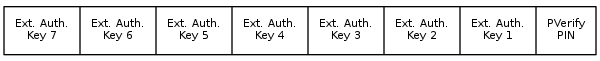
\includegraphics[width=0.75\textwidth]{image/state/securitystatebit.png}
\caption{Pembagian Fungsi Bit Security State}
\label{fig-securitystatebit}
\end{figure}

Setiap verifikasi yang berhasil akan mengubah nilai bit yang bersesuaian menjadi 1 (set). Sebaliknya ketika verifikasi gagal, nilai bit yang bersesuaian akan menjadi 0 (reset).

\item Challenge paling akhir

Challenge akan menyimpan data acak yang akan digunakan saat melakukan external authentication. Merupakan sebuah array integer 8 bit berukuran 1 block untuk algoritma kriptografi yang digunakan.

\end{enumerate}

Ketiga data/informasi ini akan disimpan sebagai sebuah state didalam sebuah struktur data dengan tipe state\_struct yang definisinya diberikan pada Listing \ref{list-statestruct}.

\begin{lstlisting}[caption={Definisi tipe struktur data state\_struct}, label={list-statestruct}]
struct state_struct
{
  uint16_t        current;     ///< pointer to current DF header
  uint8_t         securityState;  ///< security state currently active
  uint8_t         challenge[CRYPT\_BLOCK\_LEN];
};
\end{lstlisting}

\section{State Initialization}
\label{sec_stateinit}

Berfungsi menginisialisasi state manager. dipanggil setiap kali memulai sesi baru (ketika smartcard dimasukkan ke reader). Gambar \ref{fig-dfd-stateinit} menampilkan DFD dari fungsi State Initialization. Diagram alir fungsi kemudian ditampilkan pada Gambar \ref{fig-flow-stateinit}. 

\begin{figure}[h]
\centering
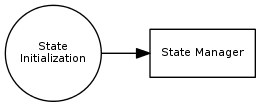
\includegraphics[width=0.5\textwidth]{image/state/dfd_stateinit.png}
\caption{DFD State Initialization}
\label{fig-dfd-stateinit}
\end{figure}

\begin{figure}[h]
\centering
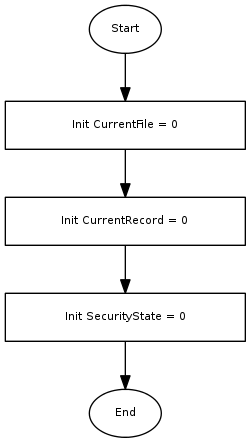
\includegraphics[height=0.5\textheight]{image/state/flow_stateinit.png}
\caption{Flowchart State Initialization}
\label{fig-flow-stateinit}
\end{figure}

\subsection {Pengujian}

\begin{table}[!h]
  \centering
  \begin{tabular}{ | c | }
    \hline
    \bf{Output} \\
    \hline
    \bf{state} \\
    \hline
    currentFile = 0 \\
    currentRecord = 0 \\
    securityState = 0x00 \\
    \hline
  \end{tabular}
  \caption{Test Vector Fungsi State Init}
  \label{tabel-test-stateinit}
\end{table}

Tabel \ref{tabel-test-stateinit} menampilkan Test Vector yang digunakan untuk menguji fungsi State Init.

\subsection {Implementasi}

Tabel \ref{tabel-stateinit} menampilkan purwarupa dari implementasi fungsi State Initialization. 

\begin{table}[!h]
  \centering
  \begin{tabular}{p{2cm} p{8cm}}
    \hline\\
    {\bf Name} & State\_Init\\
    \hline\\
    {\bf Input} & -
    \\
    \hline\\
    {\bf Output} & Result Status
    \\
    \hline
  \end{tabular}
  \caption{Prototype Fungsi State Initialization}
  \label{tabel-stateinit}
\end{table}

Listing \ref{list-stateinit} menampilkan potongan program yang mengimplementasi fungsi State Initialization

\begin{lstlisting}[caption={Listing Program Fungsi State Initialization}, label={list-stateinit}]
int State_Init()
{
  state_mng.current = 0;
  state_mng.securityState = 0;

  return STATE_OK; 
}
\end{lstlisting}


\section{Set Current File}
\label{sec_setcurrentfile}

Berfungsi Sebagai setter untuk statemember current file. Gambar \ref{fig-dfd-setcurrentfile} menampilkan DFD dari fungsi Set Current File. Diagram alir fungsi kemudian ditampilkan pada Gambar \ref{fig-flow-setcurrentfile}. 

\begin{figure}[h]
\centering
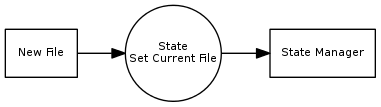
\includegraphics[width=0.75\textwidth]{image/state/dfd_setcurrentfile.png}
\caption{DFD Set Current File}
\label{fig-dfd-setcurrentfile}
\end{figure}

\begin{figure}[h]
\centering
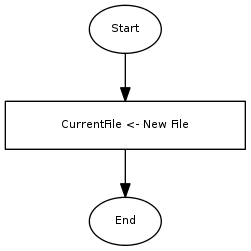
\includegraphics[height=0.25\textheight]{image/state/flow_setcurrentfile.png}
\caption{Flowchart Set Current File}
\label{fig-flow-setcurrentfile}
\end{figure}

\subsection {Pengujian}

\begin{table}[!h]
  \centering
  \begin{tabular}{ | c || c | }
    \hline
    \bf{Input} & \bf{Output} \\
    \hline
    \bf{New File} & \bf{State} \\
    \hline
    0x0000 & currentFile = 0x0000 \\
    \hline
    0x000f & currentFile = 0x000f \\
    \hline
    0x00ff & currentFile = 0x00ff \\
    \hline
    0x0fff & currentFile = 0x0fff \\
    \hline
    0xffff & currentFile = 0xffff \\
    \hline
  \end{tabular}
  \caption{Test Vector Fungsi State Set Current File}
  \label{tabel-test-setcurrentfile}
\end{table}

Tabel \ref{tabel-test-setcurrentfile} menampilkan Test Vector yang digunakan untuk menguji fungsi State Set Current File.

\subsection {Implementasi}

\begin{table}[h]
  \centering
  \begin{tabular}{p{2cm} p{8cm}}
    \hline\\
    {\bf Name} & State\_SetCurrent\\
    \hline\\
    {\bf Input} & new current file
    \\
    \hline\\
    {\bf Output} & Result Status
    \\
    \hline
  \end{tabular}
  \caption{Prototype Fungsi Set Current File}
  \label{tabel-setcurrentfile}
\end{table}

Listing \ref{list-setcurrentfile} menampilkan potongan program yang mengimplementasi fungsi Set Current File.

\begin{lstlisting}[caption={Listing Program Fungsi Set Current File}, label={list-setcurrentfile}]
int State_SetCurrent(uint16_t newFile)
{
  state_mng.current = newFile;
  state_mng.currentRecord = 0;
  state_mng.securityState = 0;

  return STATE_OK;
}
\end{lstlisting}


\section{Get Current File}
\label{sec_getcurrentfile}

Berfungsi Sebagai getter untuk state member current file. Gambar \ref{fig-dfd-getcurrentfile} menampilkan DFD dari fungsi Get Current File. Diagram alir fungsi kemudian ditampilkan pada Gambar \ref{fig-flow-getcurrentfile}. 

\begin{figure}[h]
\centering
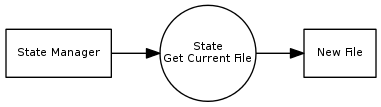
\includegraphics[width=0.75\textwidth]{image/state/dfd_getcurrentfile.png}
\caption{DFD Get Current File}
\label{fig-dfd-getcurrentfile}
\end{figure}

\begin{figure}[h]
\centering
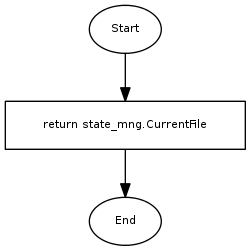
\includegraphics[height=0.25\textheight]{image/state/flow_getcurrentfile.png}
\caption{Flowchart Get Current File}
\label{fig-flow-getcurrentfile}
\end{figure}

\subsection {Pengujian}

\begin{table}[!h]
  \centering
  \begin{tabular}{ | c | }
    \hline
    \bf{Output} \\
    \hline
    \bf{Return Value} \\
    \hline
    Initialize state.currentFile to 0x0000 \\
    \hline
    = 0x0000 \\
    \hline
    Initialize state.currentFile to 0x000f \\
    \hline
    = 0x000f \\
    \hline
    Initialize state.currentFile to 0x00ff \\
    \hline
    = 0x00ff \\
    \hline
    Initialize state.currentFile to 0x0fff \\
    \hline
    = 0x0fff \\
    \hline
    Initialize state.currentFile to 0xffff \\
    \hline
    = 0xffff \\
    \hline
  \end{tabular}
  \caption{Test Vector Fungsi State Get Current File}
  \label{tabel-test-getcurrentfile}
\end{table}

Tabel \ref{tabel-test-getcurrentfile} menampilkan Test Vector yang digunakan untuk menguji fungsi State Get Current File.

\subsection {Implementasi}

Tabel \ref{tabel-getcurrentfile} menampilkan purwarupa dari implementasi fungsi Get Current File. 

\begin{table}[h]
  \centering
  \begin{tabular}{p{2cm} p{8cm}}
    \hline\\
    {\bf Name} & Get Current File\\
    \hline\\
    {\bf Input} & new current file
    \\
    \hline\\
    {\bf Output} & State Manager
    \\
    \hline
  \end{tabular}
  \caption{Prototype Fungsi Get Current File}
  \label{tabel-getcurrentfile}
\end{table}

Listing \ref{list-getcurrentfile} menampilkan potongan program yang mengimplementasi fungsi Get Current File.

\begin{lstlisting}[caption={Listing Program Fungsi Get Current File}, label={list-getcurrentfile}]
uint16_t State_GetCurrent()
{
  return state_mng.current;
}
\end{lstlisting}


\section{Get Security State}
\label{sec_getsecuritystate}

Berfungsi Sebagai getter untuk state member security state. Gambar \ref{fig-dfd-getsecuritystate} menampilkan DFD dari fungsi Get Security State. Diagram alir fungsi kemudian ditampilkan pada Gambar \ref{fig-flow-getsecuritystate}. 

\begin{figure}[h]
\centering
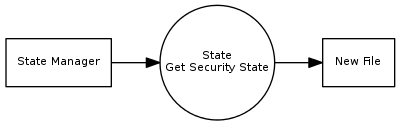
\includegraphics[width=0.5\textwidth]{image/state/dfd_getsecuritystate.png}
\caption{DFD Get Security State}
\label{fig-dfd-getsecuritystate}
\end{figure}

\begin{figure}[h]
\centering
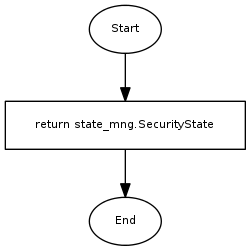
\includegraphics[height=0.25\textheight]{image/state/flow_getsecuritystate.png}
\caption{Flowchart Get Security State}
\label{fig-flow-getsecuritystate}
\end{figure}

\subsection {Pengujian}

\begin{table}[!h]
  \centering
  \begin{tabular}{ | c | }
    \hline
    \bf{Output} \\
    \hline
    \bf{Return Value} \\
    \hline
    Initialize state.securityState to 0x00 \\
    \hline
    = 0x00 \\
    \hline
    Initialize state.securityState to 0x01 \\
    \hline
    = 0x01 \\
    \hline
    Initialize state.securityState to 0x02 \\
    \hline
    = 0x02 \\
    \hline
    .... \\
    \hline
    Initialize state.securityState to 0xff \\
    \hline
    = 0xff \\
    \hline
  \end{tabular}
  \caption{Test Vector Fungsi State Get Security State}
  \label{tabel-test-getsecuritystate}
\end{table}

Tabel \ref{tabel-test-getsecuritystate} menampilkan Test Vector yang digunakan untuk menguji fungsi State Get Security State.

\subsection {Implementasi}

Tabel \ref{tabel-getsecuritystate} menampilkan purwarupa dari implementasi fungsi State Get Security State. 

\begin{table}[!h]
  \centering
  \begin{tabular}{p{2cm} p{8cm}}
    \hline\\
    {\bf Name} & State\_GetSecurityState\\
    \hline\\
    {\bf Input} & -
    \\
    \hline\\
    {\bf Output} & SecurityState
    \\
    \hline
  \end{tabular}
  \caption{Prototype Fungsi Get Security State}
  \label{tabel-getsecuritystate}
\end{table}

Listing \ref{list-getsecuritystate} menampilkan potongan program yang mengimplementasi fungsi Get Security State

\begin{lstlisting}[caption={Listing Program Fungsi Get Security State}, label={list-getsecuritystate}]
uint8_t State_GetSecurityState()
{
  return state_mng.securityState;
}
\end{lstlisting}


\section{Get Challenge}
\label{sec_getchallenge}

Berfungsi menghasilkan bilangan acak (\emph{challange}) yang digunakan untuk otentikasi eksternal. Gambar \ref{fig-dfd-getchallenge} menampilkan DFD dari fungsi Get Challenge. Diagram alir fungsi kemudian ditampilkan pada Gambar \ref{fig-flow-getchallenge}. 

\begin{figure}[h]
\centering
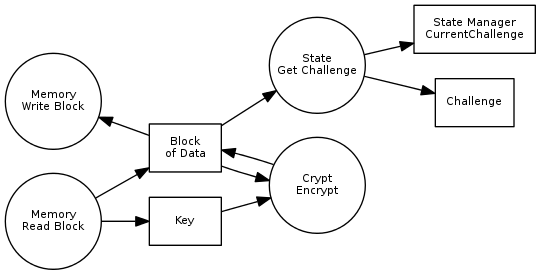
\includegraphics[width=0.75\textwidth]{image/state/dfd_getchallenge.png}
\caption{DFD Get Challenge}
\label{fig-dfd-getchallenge}
\end{figure}

\begin{figure}[!h]
\centering
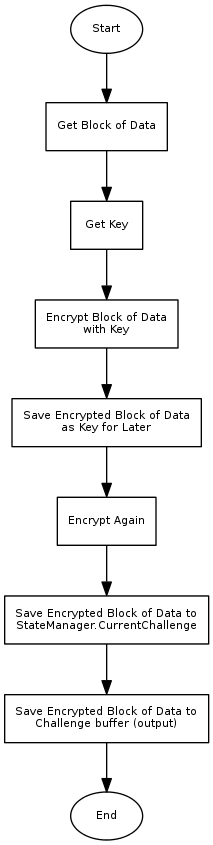
\includegraphics[height=0.75\textheight]{image/state/flow_getchallenge.png}
\caption{Flowchart Get Challenge}
\label{fig-flow-getchallenge}
\end{figure}

\subsection {Pengujian}

\begin{table}[!h]
  \centering
  \begin{tabular}{ | c | c | }
    \hline
    \multicolumn{2}{ |c| }{\bf{Output}} \\
    \hline
    \bf{challenge} & \bf{(New) Key} \\
    \hline
    \multicolumn{2}{ |c| }{Initialize data block (Memory) to 0xxxxxx} \\
    \multicolumn{2}{ |c| }{Initialize key (Memory) to 0xxxxx} \\
    \hline
    =0xxxxx & =0xxxx \\
    \hline
  \end{tabular}
  \caption{Test Vector Fungsi State Get Challenge}
  \label{tabel-test-getchallenge}
\end{table}

Tabel \ref{tabel-test-getchallenge} menampilkan Test Vector yang digunakan untuk menguji fungsi State Get Challenge.

\subsection {Implementasi}

Tabel \ref{tabel-getchallenge} menampilkan purwarupa dari implementasi fungsi Get Challenge. 

\begin{table}[h]
  \centering
  \begin{tabular}{p{2cm} p{8cm}}
    \hline\\
    {\bf Name} & State\_GetChallenge\\
    \hline\\
    {\bf Input} & 
    \\
    \hline\\
    {\bf Output} & pointer ke buffer challenge
    \\
    \hline
  \end{tabular}
  \caption{Prototype Fungsi Get Challenge}
  \label{tabel-getchallenge}
\end{table}

Listing \ref{list-getchallenge} menampilkan potongan program yang mengimplementasi fungsi Get Challenge.

\begin{lstlisting}[caption={Listing Program Fungsi Get Challenge}, label={list-getchallenge}]
void State_GetChallenge( uint8_t * buffer )
{
  iu32 block[2], key[4];

  HAL_Mem_ReadBlock( (uint16_t) SERNUM_ADDR, (uint16_t) SERNUM_LEN, (uint8_t *) block);
  /* hal_eeprom_read( (iu8*)block, SERNUM_ADDR, SERNUM_LEN ); */

  HAL_Mem_ReadBlock( (uint16_t) RAND_STATE_ADDR, (uint16_t) sizeof(key), (uint8_t *) key);
  /* hal_eeprom_read( (iu8*)key, RAND_STATE_ADDR, sizeof(key) ) */

  key[2]=key[1];
  key[3]=key[0];

  crypt_enc( block, key );

  HAL_Mem_WriteBlock( (uint16_t) RAND_STATE_ADDR, (uint16_t) RAND_STATE_LEN, (uint8_t *) block);

  crypt_enc( block, key );

  memcpy( state_mng.challenge, block, sizeof(block) );

  memcpy( buffer, block, CRYPT_BLOCK_LEN );
}
\end{lstlisting}


\section{Verify (PIN)}
\label{sec_verify}

Berfungsi untuk otentikasi dasar menggunakan PIN. Gambar \ref{fig-dfd-verify} menampilkan DFD dari fungsi State Verify. Diagram alir fungsi kemudian ditampilkan pada Gambar \ref{fig-flow-verify}. 

\begin{figure}[h]
\centering
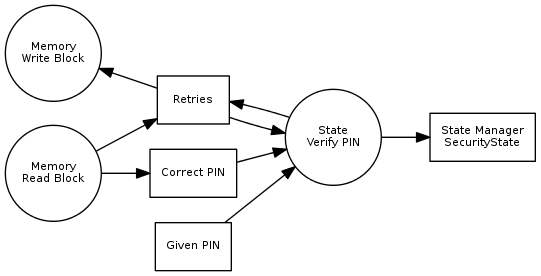
\includegraphics[width=0.75\textwidth]{image/state/dfd_verify.png}
\caption{DFD Verify PIN}
\label{fig-dfd-verify}
\end{figure}

\begin{figure}[!h]
\centering
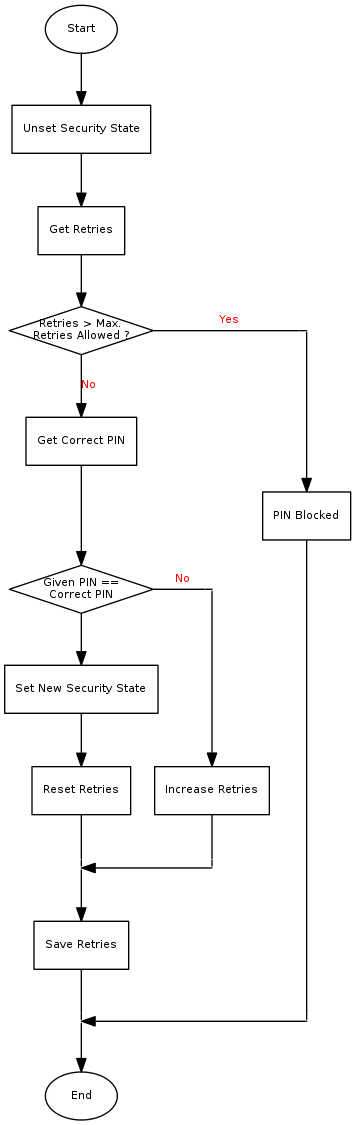
\includegraphics[height=0.9\textheight]{image/state/flow_verify.png}
\caption{Flowchart Verify PIN}
\label{fig-flow-verify}
\end{figure}

\subsection {Pengujian}

\begin{table}[!h]
  \centering
  \begin{tabular}{ | c || c | c| c | }
    \hline
    \bf{Input} & \multicolumn{3}{ c| }{\bf{Output}} \\
    \hline
    \bf{Given PIN} & \bf{State} & \bf{Retries} & \bf{Ret. Value} \\
    \hline
    \multicolumn{4}{ |c| }{Initialize PIN (Memory) to 0x1234} \\
    \multicolumn{4}{ |c| }{Initialize Retries (Memory) to 0} \\
    \multicolumn{4}{ |c| }{Initialize SecurityState (State) to 0} \\
    \hline
    0x1234 & =1 & =0 & =STATE\_OK \\
    \hline
    0x1111 & =0 & =1 & =STATE\_WRONG \\
    \hline
    0x1111 & =0 & =2 & =STATE\_WRONG \\
    \hline
    0x1111 & =0 & =3 & =STATE\_WRONG \\
    \hline
    0x1111 & =0 & =3 & =STATE\_BLOCK \\
    \hline
  \end{tabular}
  \caption{Test Vector Fungsi State Verify}
  \label{tabel-test-verify}
\end{table}

Tabel \ref{tabel-test-verify} menampilkan Test Vector yang digunakan untuk menguji fungsi State Verify (PIN).

\subsection {Implementasi}

Tabel \ref{tabel-verify} menampilkan purwarupa dari implementasi fungsi Verify PIN. 

\begin{table}[h]
  \centering
  \begin{tabular}{p{2cm} p{8cm}}
    \hline\\
    {\bf Name} & State\_Verify\\
    \hline\\
    {\bf Input} & PIN
    \\
    \hline\\
    {\bf Output} & Result Status
    \\
    \hline
  \end{tabular}
  \caption{Prototype Fungsi Verify}
  \label{tabel-verify}
\end{table}

Listing \ref{list-verify} menampilkan potongan program yang mengimplementasi fungsi Verify.

\begin{lstlisting}[caption={Listing Program Fungsi Verify}, label={list-verify}]
int State_Verify(uint8_t *pin)
{
  state_mng.securityState &= 0xfe;

  uint8_t retries;

  retries = HAL_Mem_ReadByte(PIN_RETRIES_ADDR);

  if (retries > PIN_MAX_RETRIES)
    {
      return STATE_BLOCKED;
    }

  uint8_t i, temp, diff=0;
  for( i=0; i<PIN_LEN; i++ )
    {
      temp = HAL_Mem_ReadByte(PIN_ADDR+i);
      /* HAL_IO_TxByte(pin[i]); */
      /* HAL_IO_TxByte(temp); */
      diff |= temp^pin[i];
    }

  if( diff>0 )
    {
      retries++;
    }
  else
    {
      retries=0;
    }

  HAL_Mem_WriteByte(PIN_RETRIES_ADDR, retries);
  
  if( diff>0 )
    {
      return STATE_WRONG;
    }

  state_mng.securityState |= 0x01;

  return STATE_OK;
}
\end{lstlisting}

\section{Verify Auth}
\label{sec_verifyauth}

Berfungsi untuk verifikasi user lanjutan menggunakan metode otentikasi. Gambar \ref{fig-dfd-verifyauth} menampilkan DFD dari fungsi State Verify Key. Diagram alir fungsi kemudian ditampilkan pada Gambar \ref{fig-flow-verifyauth}. 

\begin{figure}[h]
\centering
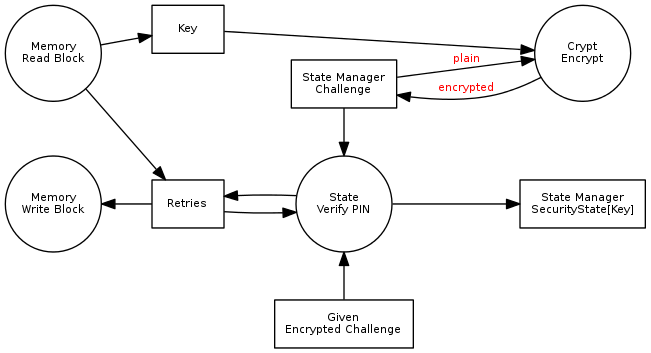
\includegraphics[width=0.75\textwidth]{image/state/dfd_verifykey.png}
\caption{DFD Verify Auth}
\label{fig-dfd-verifyauth}
\end{figure}

\begin{figure}[!h]
\centering
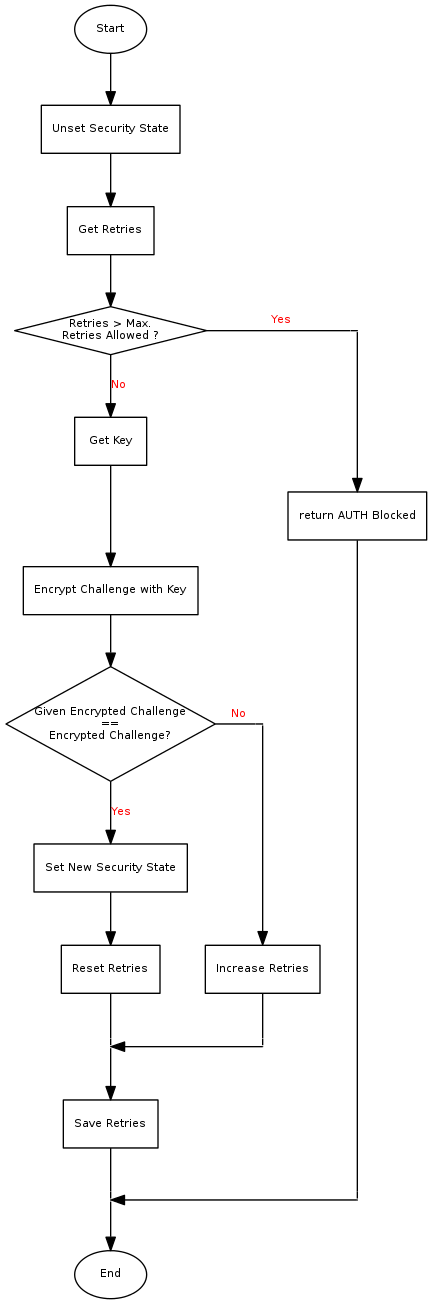
\includegraphics[height=0.9\textheight]{image/state/flow_verifykey.png}
\caption{Flowchart Verify Auth}
\label{fig-flow-verifyauth}
\end{figure}

\subsection {Pengujian}

\begin{table}[!h]
  \centering
  \begin{tabular}{ | c || c | c | c | }
    \hline
    \bf{Input} & \multicolumn{3}{ c| }{\bf{Output}} \\
    \hline
    \bf{Given Enc. Challenge} & \bf{State} & \bf{Retries} & \bf{Ret. Value} \\
    \hline
    \multicolumn{4}{ |c| }{Initialize Key (Memory) to 0xxxxx} \\
    \multicolumn{4}{ |c| }{Initialize Retries (Memory) to 0} \\
    \multicolumn{4}{ |c| }{Initialize Challenge (State) to 0} \\
    \multicolumn{4}{ |c| }{Initialize SecurityState (State) to 0} \\
    \hline
    =0xxxxx & =1 & =0 & =STATE\_OK \\
    \hline
    =0xxxxx & =0 & =1 & =STATE\_WRONG \\
    \hline
    =0xxxxx & =0 & =2 & =STATE\_WRONG \\
    \hline
    =0xxxxx & =0 & =3 & =STATE\_WRONG \\
    \hline
    =0xxxxx & =0 & =3 & =STATE\_BLOCK \\
    \hline
  \end{tabular}
  \caption{Test Vector Fungsi State Verify Auth}
  \label{tabel-test-verifyauth}
\end{table}

Tabel \ref{tabel-test-verifyauth} menampilkan Test Vector yang digunakan untuk menguji fungsi State Verify Auth.

\subsection {Implementasi}

Tabel \ref{tabel-verifyauth} menampilkan purwarupa dari implementasi fungsi Verify Auth. 

\begin{table}[h]
  \centering
  \begin{tabular}{p{2cm} p{8cm}}
    \hline\\
    {\bf Name} & State\_VerifyAuth\\
    \hline\\
    {\bf Input} & Encrypted Challenge
    \\
    \hline\\
    {\bf Output} & Result Status
    \\
    \hline
  \end{tabular}
  \caption{Prototype Fungsi Verify Auth}
  \label{tabel-verifyauth}
\end{table}

Listing \ref{list-verifyauth} menampilkan potongan program yang mengimplementasi fungsi Verify Auth

\begin{lstlisting}[caption={Listing Program Fungsi Verify Auth}, label={list-verifyauth}]
uint8_t State_VerifyAuth( uint8_t * encrypted )
{
  uint8_t retries;
  retries = HAL_Mem_ReadByte(EXT_AUTH_RETRIES_ADDR);

  if (retries > EXT_AUTH_MAX_RETRIES)
    {
      return STATE_BLOCKED;
    }

  uint32_t key[4];
  HAL_Mem_ReadBlock( (uint16_t) EXT_AUTH_KEY_ADDR, (uint16_t) EXT_AUTH_KEY_LEN, (uint8_t *) key);

  crypt_enc( state_mng.challenge, key );

  /* Compare result */
  if( memcmp( encrypted, state_mng.challenge, CRYPT_BLOCK_LEN ) ) {
    retries++;
    HAL_Mem_WriteByte(EXT_AUTH_RETRIES_ADDR, retries);

    return STATE_WRONG;
  }

  if(retries > 0)
    {
      retries = 0;
      HAL_Mem_WriteByte(EXT_AUTH_RETRIES_ADDR, retries);
    }

  state_mng.securityState |= 0x02;

  return STATE_OK;
}
\end{lstlisting}

